\documentclass[a4paper]{article}
\usepackage{amsmath}
\usepackage[makeroom]{cancel}
%\usepackage{pdffig}
%\usepackage{subfigure}
\usepackage{graphicx}
\usepackage{amsfonts}
\usepackage{amsmath}
\usepackage{amssymb}
\usepackage{color}
\usepackage{pstricks}
\usepackage{float}
\usepackage{listings}
\usepackage{color} %red, green, blue, yellow, cyan, magenta, black, white
\definecolor{mygreen}{RGB}{28,172,0} % color values Red, Green, Blue
\definecolor{mylilas}{RGB}{170,55,241}

\date{\today}
\setlength{\topmargin}{-12.5mm}
\setlength{\textwidth}{7in}
\setlength{\oddsidemargin}{-8mm}
\setlength{\textheight}{9.25in}
\setlength{\footskip}{0.8in}
\usepackage{fancyhdr}
\pagestyle{fancy}
\lhead{ECEN-5523: Estimation Theory}
\rhead{}
\cfoot{\thepage}
\rfoot{}
\title{Estimation Theory -ECEN 5523 \\Reaction Wheel Pendulum Filter Design Project}
\author{GIRISH JOSHI}
\begin{document}
	\maketitle
\fontsize{12}{14}
\selectfont

\lstset{language=Matlab,%
	%basicstyle=\color{red},
	breaklines=true,%
	morekeywords={matlab2tikz},
	keywordstyle=\color{blue},%
	morekeywords=[2]{1}, keywordstyle=[2]{\color{black}},
	identifierstyle=\color{black},%
	stringstyle=\color{mylilas},
	commentstyle=\color{mygreen},%
	showstringspaces=false,%without this there will be a symbol in the places where there is a space
	numbers=left,%
	numberstyle={\tiny \color{black}},% size of the numbers
	numbersep=9pt, % this defines how far the numbers are from the text
	emph=[1]{for,end,break},emphstyle=[1]\color{red}, %some words to emphasise
	%emph=[2]{word1,word2}, emphstyle=[2]{style},    
}

\section{Reaction Wheel Pendulum: Model}
The Reaction Wheel Pendulum, is a simple pendulum with a rotating wheel at the end. The wheel is actuated by a motor mounted on the pendulum. This motor can produce a torque on the wheel, causing
the wheel to spin. According to Newton’s third law, there is an equal and opposite
reaction torque on the pendulum due to conservation of the angular of momentum principle. This reaction torque can be
used to control the motion of the pendulum.\\

The parameters of the Reaction Wheel Pendulum system are given as:
\begin{itemize}
	\item $m_p$ = Mass of pendulum
	\item $m_r$ = Mass of rotor
	\item $m = m_p+m_r$ = Combined mass of rotor and pendulum
	\item $J_p$ = Moment of inertia of the pendulumabout its center of mass
	\item $J_r$ = Moment of inertia of the rotor about its center of mass
	\item $l_p$ = Distance from pivot to the center of mass of the pendulum
	\item $l_r$ = Distance from pivot to the center of mass of the rotor
	\item $l$ = Distance from pivot to the center of mass of pendulumand rotor
	\item $\theta$ = Angle of pendulum
	\item $\theta_r$ = Angle of rotor
	\item $\theta_m = \theta_r-\theta$ = Angle of motor
\end{itemize}
The equation of motion of Reaction wheel pendulum can be derived from lagrangian principle. The Lagrangian is defined as the difference between the kinetic and potential energy of the system.
\begin{equation}
L(\theta,\dot \theta,\theta_r,\dot \theta_r) = K.E-P.E
\end{equation}
for pendulum the lagrangian can be written as,
\begin{equation}
L_p(\theta , \dot \theta) = \frac{1}{2}J\theta^2 - mgl(1-cos(\theta))
\label{eq:1}
\end{equation}
and Lagrangian for the rotor can be written as 
\begin{equation}
L_r(\theta_r , \dot \theta_r) = \frac{1}{2}J_r\theta_r^2
\label{eq:2}
\end{equation}
The Lagrange equation of motion, for Reaction wheel pendulum can be written as,
\begin{equation}
\frac{\partial}{\partial t}\left(\frac{\partial L_p}{\partial \dot \theta}\right) - \left(\frac{\partial L_p}{\partial \theta}\right) = \tau
\label{eq:3}
\end{equation}
\begin{equation}
\frac{\partial}{\partial t}\left(\frac{\partial L_r}{\partial \dot \theta_r}\right) - \left(\frac{\partial L_r}{\partial \theta_r}\right) = \tau
\label{eq:4}
\end{equation}
Using expression \ref{eq:1} and \ref{eq:2} in \ref{eq:3} and \ref{eq:4} the equation of motion for the reaction wheeel pendulum can be written  as
\begin{equation}
J\ddot{\theta}+mglsin(\theta) = -\tau
\label{eq:5}
\end{equation}
\begin{equation}
J_r\ddot{\theta_r} = \tau
\label{eq:6}
\end{equation}
The control torque on the pendulum is generated using the motor connected to the rotor. The torque expression for the motor is given as follows,
\begin{equation}
\tau = k_ti
\label{eq:7}
\end{equation}
where $\tau$ is the reaction torque generated by the motor, $K_t$ is torque constant and $i$ is armature current. The armature current is the function of the voltage applied across the motor coils and back emf generated due to motor coils cutting through the magnetic field of stator magnets.
\begin{equation}
Ri = e-K_b\dot \theta_m
\label{eq:8}
\end{equation}
Using \ref{eq:7} and \ref{eq:8}, non-linear equation of motion of reaction wheel pendulum \ref{eq:5} and \ref{eq:6} can be written in state space form as follows.
\begin{equation}
\ddot{\theta} = \frac{-mglsin(\theta)}{g}-\frac{K_tK_b}{JR}\dot \theta + \frac{K_tK_b}{JR}\dot \theta_r-\frac{K_te}{JR}
\label{eq:9}
\end{equation}
\begin{equation}
\ddot{\theta_r} = \frac{K_tK_b}{J_rR}\dot \theta - \frac{K_tK_b}{J_rR}\dot \theta_r + \frac{K_te}{J_rR}
\label{eq:10}
\end{equation}
\subsection{Linearization of Equation of Motion}
The nonlinear equation of motion for the reaction wheel pendulum \ref{eq:9}, \ref{eq:10} can be written as
\begin{equation}
\ddot{\theta} = g_1(\theta,\dot \theta,\theta_r,\dot \theta_r)
\label{eq:11}
\end{equation}
\begin{equation}
\ddot{\theta_r} = g_2(\theta,\dot \theta,\theta_r,\dot \theta_r)
\label{eq:12}
\end{equation}
Defining the state variable as follows $\theta_1 = \theta$, $\theta_2 = \dot \theta$, $\theta_3 = \theta_r$ and $\theta_4 = \dot \theta_r$, expression \ref{eq:11} and \ref{eq:12} is written in state space form, 
\begin{eqnarray}
\dot{\theta_1} &=& f_1(\theta_2) = \theta_2 \label{eq:13}\\
\dot{\theta_2} &=& f_2(\theta_1,\theta_2,\theta_3,\theta_4) \label{eq:14}\\
\dot{\theta_3} &=& f_3(\theta_4) =  \theta_4 \label{eq:15} \\
\dot{\theta_4} &=& f_4(\theta_1,\theta_2,\theta_3,\theta_4) \label{eq:16}
\end{eqnarray}
Using the first order Taylor series approximation, the state space form of nonlinear equation \ref{eq:13} to \ref{eq:16} can be written in the Linearized form as follows linearized about the equilibrium point $\theta = 0$,
\begin{eqnarray}
\dot X &=& AX+BU \label{eq:19}\\
Y &=& HX+DU \label{eq:20}
\end{eqnarray}
where
\begin{equation}
A = \left[\begin{array}{cccc}
\frac{\partial f_1}{\partial \theta_1}& \frac{\partial f_1}{\partial \theta_2}  &  \frac{\partial f_1}{\partial \theta_3}  & \frac{\partial f_1}{\partial \theta_4}  \\ 
&&&\\
\frac{\partial f_2}{\partial \theta_1}& \frac{\partial f_2}{\partial \theta_2}  &  \frac{\partial f_2}{\partial \theta_3}  & \frac{\partial f_2}{\partial \theta_4}  \\  
&&&\\
\frac{\partial f_3}{\partial \theta_1}& \frac{\partial f_3}{\partial \theta_2}  &  \frac{\partial f_3}{\partial \theta_3}  & \frac{\partial f_3}{\partial \theta_4}  \\ 
&&&\\
\frac{\partial f_4}{\partial \theta_1}& \frac{\partial f_4}{\partial \theta_2}  &  \frac{\partial f_4}{\partial \theta_3}  & \frac{\partial f_4}{\partial \theta_4}  \\  
\end{array} \right]
\end{equation}\\
\begin{equation}
B = \left[\begin{array}{c}
\frac{\partial f_1}{\partial e}\\ 
\\
\frac{\partial f_2}{\partial e}\\ 
\\
\frac{\partial f_3}{\partial e}\\ 
\\
\frac{\partial f_4}{\partial e}
\end{array}\right]
\end{equation}
There by the state space model for reaction wheel pendulum can be written as,
\begin{equation}
\left[\begin{array}{c}
\dot \theta_1\\ 
\dot \theta_2\\ 
\dot \theta_3\\ 
\dot \theta_4
\end{array}\right] = \left[\begin{array}{cccc}
0& 1 & 0  &0  \\ 
\frac{-mgl}{g}& -\frac{K_tK_b}{JR} & 0 & \frac{K_tK_b}{JR}  \\ 
0& 0 & 0 & 1  \\ 
0 & \frac{K_tK_b}{JR}  & 0 &-\frac{K_tK_b}{JR}
\end{array} \right]\left[\begin{array}{c}
\theta_1\\ 
\theta_2\\ 
\theta_3\\ 
\theta_4
\end{array}\right] + \left[\begin{array}{c}
0\\ 
-\frac{K_t}{JR}\\ 
0\\ 
\frac{K_t}{J_rR}
\end{array}\right]e
\end{equation} 
\begin{equation}
Z = \left[\begin{array}{cccc}
1 & 0 & 0 & 0  \\ 
-1& 0 & 1 & 0 
\end{array} \right]\left[\begin{array}{c}
\theta_1\\ 
\theta_2\\ 
\theta_3\\ 
\theta_4
\end{array}\right]
\end{equation}
\begin{figure}[h]
\centering
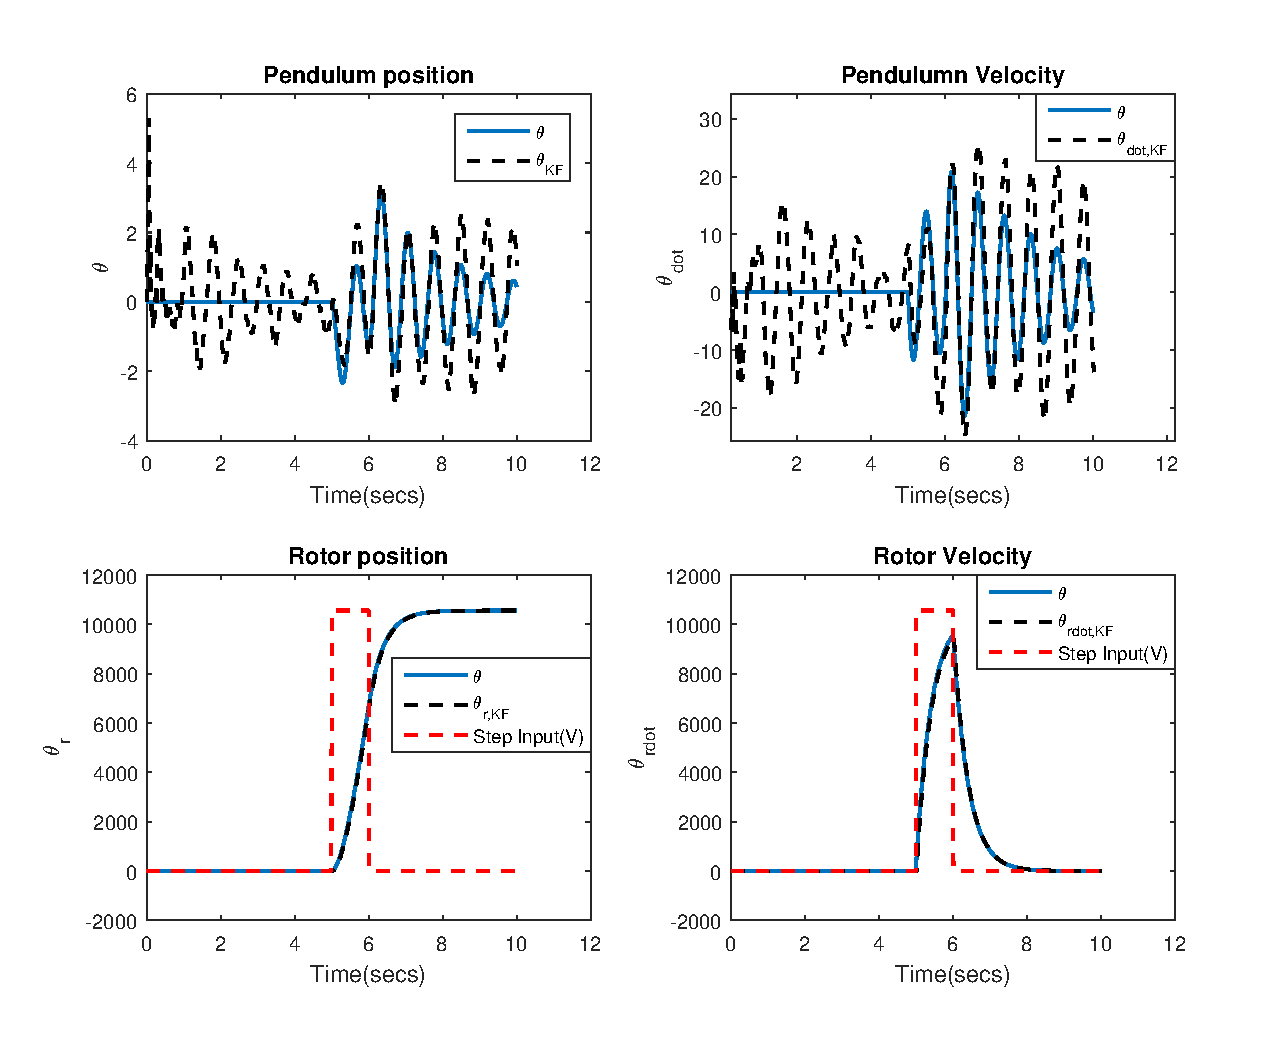
\includegraphics[width=0.7\linewidth]{fig/plot_1}
\caption{Linear plant model, Simulation with Motor Step Input}
\label{fig:plot_1}
\end{figure}
\newpage
\section{Angular Sensors}
A Precision Hall Effect Angle Sensor ``A1332" from $Allegro^{TM}$ Microsystems is chosen for the angle measurement of the pendulum, the specification sheet of the sensor is provided in the Annexure.\\
The sensor noise distribution specification at different operating temperature is given following Figure \ref{fig:Sensor_noise}.
The Sensor measurement Noise Specification (from the Figure\ref{fig:Sensor_noise})\\
\begin{center}
	\begin{tabular}{|c|c|}
		\hline  & Specification \\ 
		\hline Measurement Bias & $0.3^0$ \\ 
		\hline $\pm 3\sigma $Standard Deviation & $0.2^0$  \\ 
		\hline Variance $\sigma^2$ & 0.0044 \\ 
		\hline 
	\end{tabular} 
\end{center}

\begin{figure}[h!]
\centering
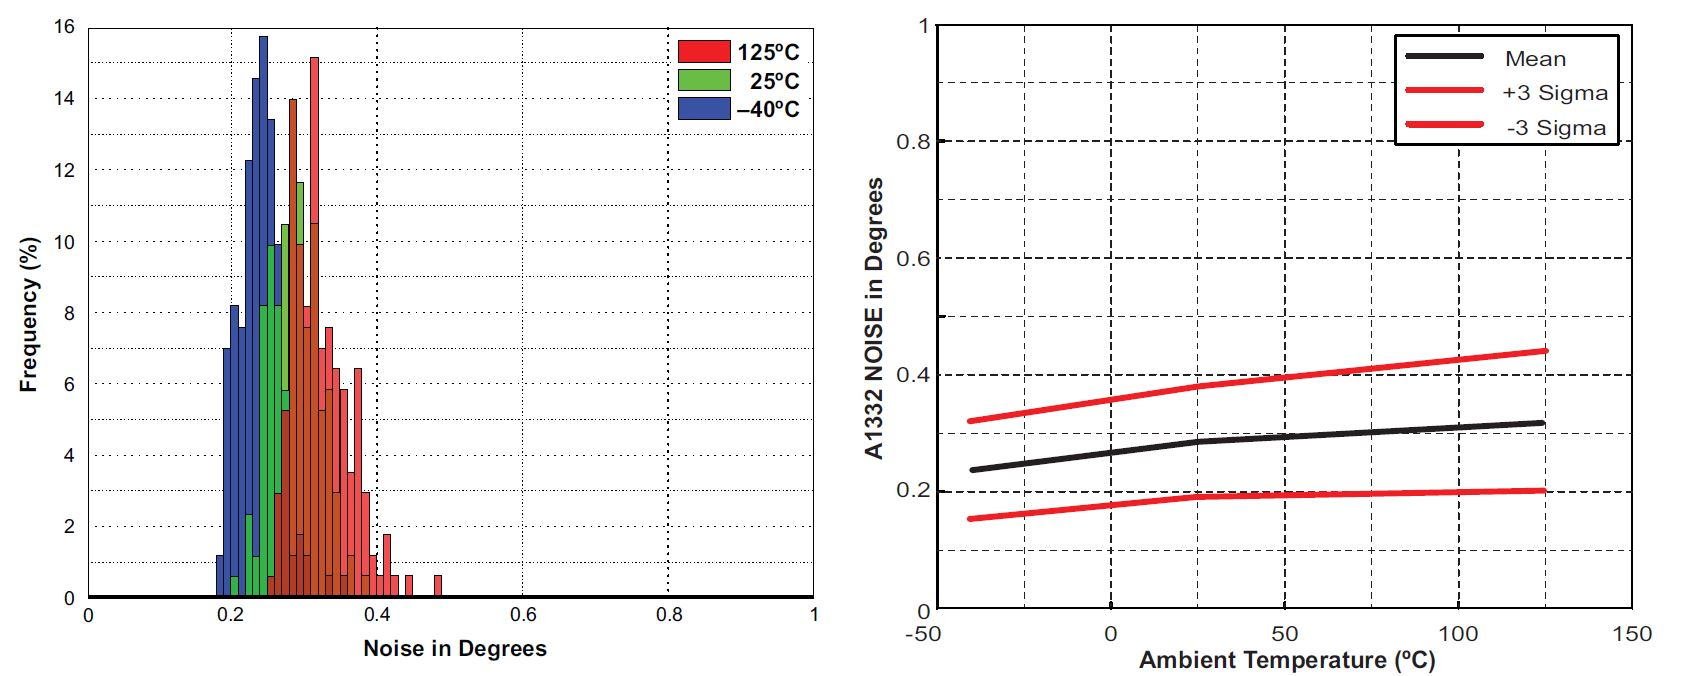
\includegraphics[width=0.625\linewidth]{fig/Sensor_noise}
\caption{Hall Effect Angle Sensor measurement Noise Distribution vs. operating Temperature}
\label{fig:Sensor_noise}
\end{figure}
\section{Filtering}
In this project, the results are presented for estimation of the state vector of the reaction wheel pendulum through Kalman and Extended Kalman filtering. The details of the filter development, filter equation and corresponding results are presented in the subsequent sections.
\subsection{Kalman Filtering}
In this section details are presented for the Linearized Discrete Kalman Filtering to estimate the state of the Reaction wheel pendulum plant.
For Discrete Kalman Filtering(DKF) the linearized plant model needs to be written in the discrete form. The discretization of the linear continues time model for DKF is carried out as follows.\\
The discrete time model of the system can be written as,
\begin{eqnarray}
X(k+1) &=& \Phi X(k) + \Psi U(k) \label{eq:17}\\
Z(k+1) &=& HX(k+1) \label{eq:18}
\end{eqnarray}  
The value of the state transition matrices $\Phi$,control effective matrix $\Psi$ needs to be determined. While they are independent of the time $T$ and constant, they depend on the value of the sampling interval $dt$.\\
The solution of the continues time state equation \ref{eq:19} and \ref{eq:20} for time $kT$ and $(k+1)T$ can be written as
\begin{eqnarray}
X(kT) &=& e^{AkT}X(0) + e^{AkT}\int_{0}^{kT} e^{-A\tau}BU(\tau)d\tau \label{eq:21}\\
X((k+1)T) &=& e^{A(k+1)T}X(0) + e^{A(k+1)T}\int_{kT}^{(k+1)T} e^{-A\tau}BU(\tau)d\tau \label{eq:22}
\end{eqnarray}
multiplying \ref{eq:21} by $e^{AT}$ and solving for $e^{A(k+1)T}X(0)$ and further substituting this expression in \ref{eq:22}, the expression $X((k+1)T)$ can written as function of $X(kT)$ as follows
\begin{equation}
X((k+1)T) = e^{A(k+1)T}X(k) + \int_{kT}^{(k+1)T} e^{(A(k+1)T-\tau)}BU(kT)d\tau
\label{eq:23}
\end{equation}
Now we see that as $\tau$ ranges from kT to (k + 1)T. Defining a new variable $\lambda = (k +1)T-\tau$ .
Therefore $ d\lambda = -d\tau$ and $\lambda$ ranges from T to 0 as $\tau$ ranges from kT to (k + 1)T. Thus we \ref{eq:23} can be written as
\begin{equation}
X((k+1)T) = e^{AT}X(k) + \int_{0}^{T} e^{(A\lambda)}BU(kT)d\lambda
\label{eq:24}
\end{equation}
Therefore equating \ref{eq:17} and \ref{eq:24} we can write discrete system state transition matrix as follows,
\begin{eqnarray}
\Phi &=& e^{AT} \label{eq:25}\\
\Psi &=& \int_{0}^{T} e^{(A\lambda)}d\lambda B \label{eq:26}
\end{eqnarray}
where $T$ is sampling time.\\
With the discrete time system definition the kalman filtering state estimation equation can be written as \\
\begin{center}
	\begin{tabular}{|c|c|}
		\hline & \\
		 Model & Dynamics  \\
		             & $\dot X = f(x,U,W)$\\
		             & Measurement Equation\\
		             & $Z(k+1) = HX(k+1)$ \\
		\hline & \\             
		 Initialization & $\hat X(k|k) = \hat X(0)$\\ 
		                      & Error Covariance\\
		                      & $P(k|k) = E(\tilde X(0) \tilde X(0)^T )$\\
		\hline & \\
		  State & $\hat X(k+1|k) = \Phi \hat X(k|k) + \Psi U(k)$  \\ 
		  Prediction & \\
		\hline & \\
		  Covarince & $P(k+1|k) = \Phi P(k|k)\Phi ^T + \Gamma Q \Gamma ^T$  \\ 
		  propagation & \\
		\hline  &  \\ 
		  Kalman  & $K(k+1) = P(k+1|k)H^T(HP(k+1|k)H^T+R)^{-1}$ \\
	      Gain Computation            	& \\
		\hline  &  \\
		  State Update & $\hat X(k+1|k+1) = \hat X(k+1|k) + K(k+1)(Z(k+1)-H\hat X(k+1|k))$\\
		        &  \\ 
		\hline  &  \\ 
		  Covariance Update & $P(k+1|k+1) = (I-KH)P(k+1|k)(I-KH)^T + KRK^T$\\
		       &  or \\
		       & $P(k+1|k+1) = (I-KH)P(k+1|k)$ \\
		\hline
		
	\end{tabular} 
\end{center}
Assuming the Parameters for reaction wheel pendulum as follows
\begin{itemize}
\item $m_p = 0.2164$ kg
\item $J_p = 2.233 \times 10^{-4}kgm^2 $ 
\item $m_r = 0.0850$kg
\item $J_r = 2.495 \times 10^{-5}kgm^2$ 
\item $m = 0.3014$ kg
\item $l = 0.1200$ m
\item $l_p = 0.1173$ m
\item $l_r = 0.1270$ m
\item $J = 4.572 x 10^{-3}kgm^2$ 
\end{itemize}
The Linear discretized plant model for reaction wheel pendulum can be written as follows
\begin{equation}
\left[\begin{array}{c}
\theta_1(k+1)\\ 
\theta_2(k+1)\\ 
\theta_3(k+1)\\ 
\theta_4(k+1)
\end{array}\right] = \left[\begin{array}{cccc}
    0.9961 &   0.0100   &      0  &  0.0000\\
    -0.7750  &  0.9960  &       0  &  0.0001\\
    -0.0000  &  0.0001  &  1.0000  &  0.0099\\
    -0.0096  &  0.0245  &       0  &  0.9754
\end{array} \right]\left[\begin{array}{c}
\theta_1(k\\ 
\theta_2(k)\\ 
\theta_3(k)\\ 
\theta_4(k)
\end{array}\right]+\left[\begin{array}{c}
-0.0000\\
-0.0048\\
0.0089\\
0.8852
\end{array} \right]e 
\end{equation}
The measurement vector consists encoder measurement of the absolute angle of the pendulum and motor rotation. Therefore the measurement equation is written as
\begin{equation}
Z(k+1) = \left[\begin{array}{cccc}
 1   &  0   &  0  &   0 \\
 -1  &   0   &  1   &  0
\end{array} \right]\left[\begin{array}{c}
\theta_1(k+1)\\ 
\theta_2(k+1)\\ 
\theta_3(k+1)\\ 
\theta_4(k+1)
\end{array}\right]
\end{equation}
The Noise covariance matrix $R$ is designed based on the sensor specification,
\begin{equation}
R = \left[\begin{array}{cc}
0.04^0&0  \\ 
0& 0.04^0
\end{array}\right] 
\end{equation}
and process noise covariance $Q$ is tuned for the optimum performance of the filter,
\begin{equation}
Q = \left[\begin{array}{cc}
1e-4&0  \\ 
0& 1e-4
\end{array}\right] 
\end{equation}
\subsubsection{Results: Kalman Filtering}
Matlab ``ODE-45" integration is used for simulating the actual plant model for Reaction Wheel Pendulum. The $dt$ for the simulation is chosen as $\frac{1}{10}^{th}$ of the inverse fo the highest eigen value of the continues time, linear state transition matrix.\\
the continues time state equation can be written as,
\begin{equation}
\left[\begin{array}{c}
\dot \theta_1\\ 
\dot \theta_2\\ 
\dot \theta_3\\ 
\dot \theta_4
\end{array}\right] = \left[\begin{array}{cccc}
         0  &  1.0000    &     0   &      0\\
         -77.6046 &  -0.0136   &      0  &  0.0136\\
         0    &     0    &     0   & 1.0000\\
         0  &  2.4868   &      0  & -2.4868
\end{array} \right]\left[\begin{array}{c}
\theta_1\\ 
\theta_2\\ 
\theta_3\\ 
\theta_4
\end{array}\right]+\left[\begin{array}{c}
0\\
-0.4953\\
0\\
90.7600
\end{array} \right]e 
\end{equation}\\

$dt$ for the simulation is \[dt = \frac{1}{10*max(||[Re(\lambda_i)]||)} = \frac{1}{10*2.5} = 0.04secs\]\\

The figure \ref{fig:plot_1_kf1} shows the kalman filter performance for pendulum initial condition much away from the equilibrium point. The motor input, a pulse of voltage is also applied to the motor at $t = 5secs$. It can be observed that the kalman filter estimates are not accurate enough, due to linearization error as we are operating in the region away from the equilibrium point.\\

Simulation in figure \ref{fig:plot_1_kf2} demonstrates that system can be put into oscillation using external input to motor. The pendulum is at placed at its equilibrium position to start with and motor voltage $V = 1volts$ is applied for $1sec$ starting from $t =5secs$. Due to the torque generated by the motor the pendulum is set in oscillations. Since the pendulum oscillates in the neighborhood of the equilibrium points, after initial transient error settles, the Linearized Kalman filter estimates does good in state estimation. \\

Figure \ref{fig:plot_1_kf3} simulates the system with no external inputs. The pendulum is initially displaced to very small angle $\theta_1 = 3^0$ and released to freely oscillate under the influence of the gravity. Since the peak oscillation angles are with in the close neighborhood of the equilibrium point, the performance of the ``Linearized Kamlan filter" in estimating the state of the pendulum and rotor is good.    
\begin{figure}
\centering
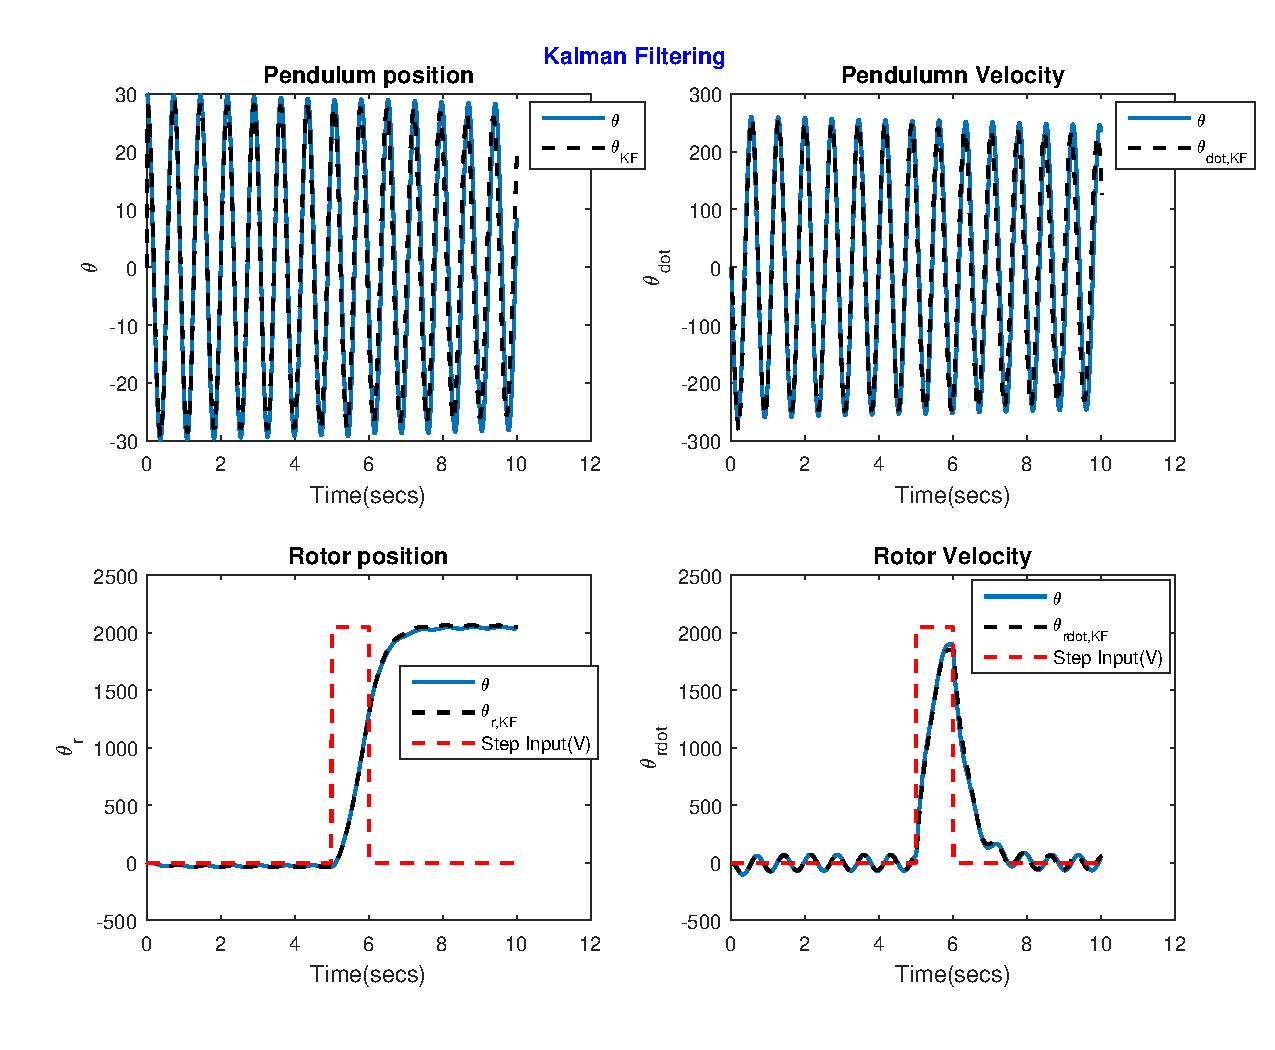
\includegraphics[width=0.7\linewidth]{fig/plot_1_kf1}
\caption{Initial Condition: $\theta_1 = 30^0$, $\theta_2 = 0$ and motor pulse of 5V is applied at $t = 5secs$}
\label{fig:plot_1_kf1}
\end{figure}
\begin{figure}
\centering
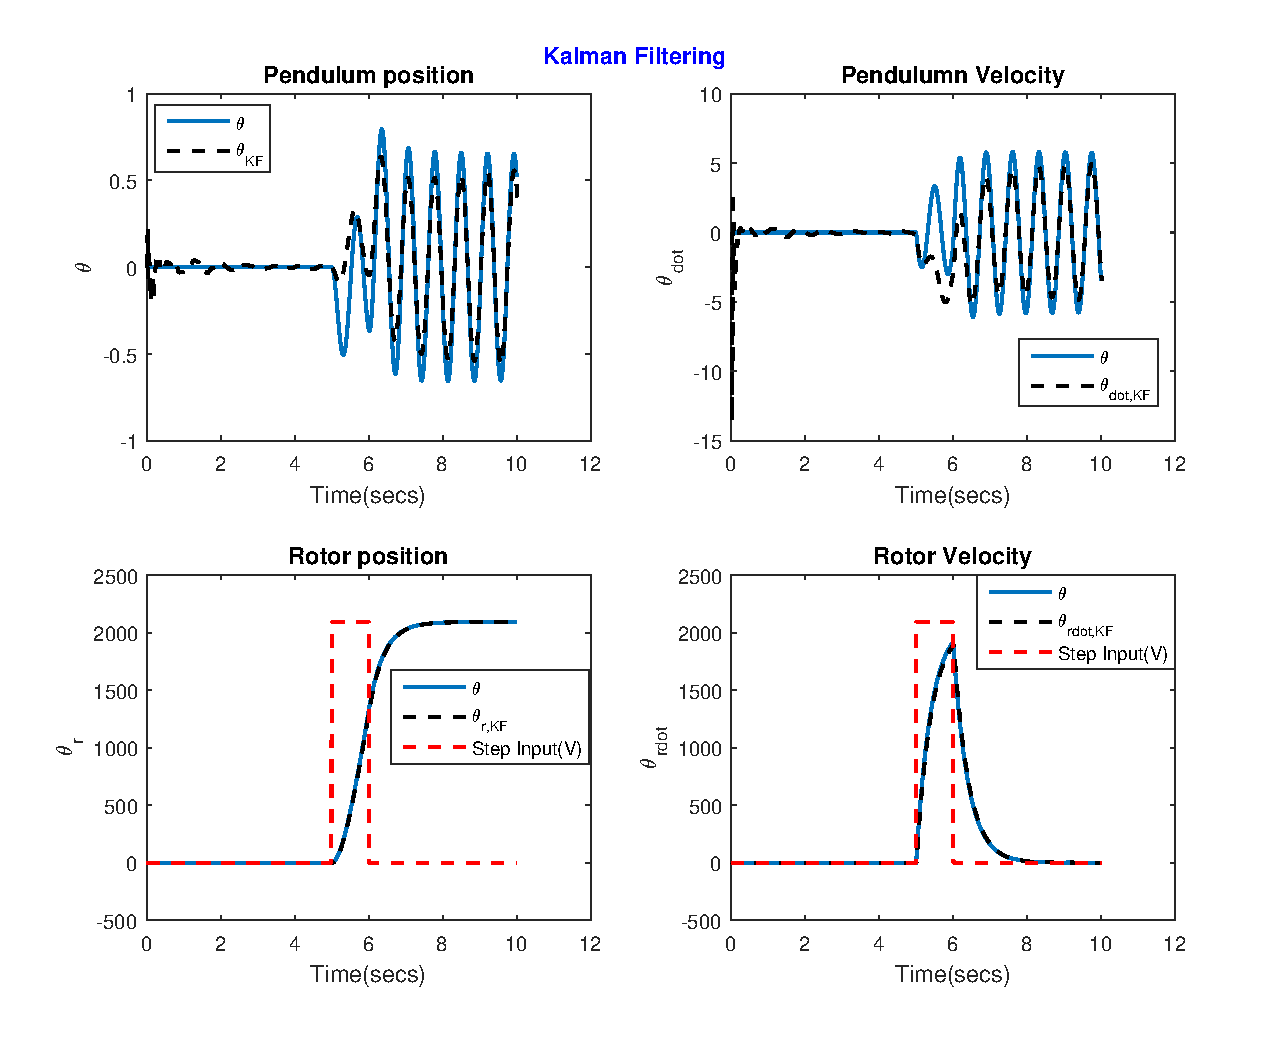
\includegraphics[width=0.7\linewidth]{fig/plot_1_kf2}
\caption{Initial Condition: $\theta_1 = 0$, $\theta_2 = 0$ and motor pulse of 5V is applied at $t = 5secs$}
\label{fig:plot_1_kf2}
\end{figure}
\begin{figure}
	\centering
	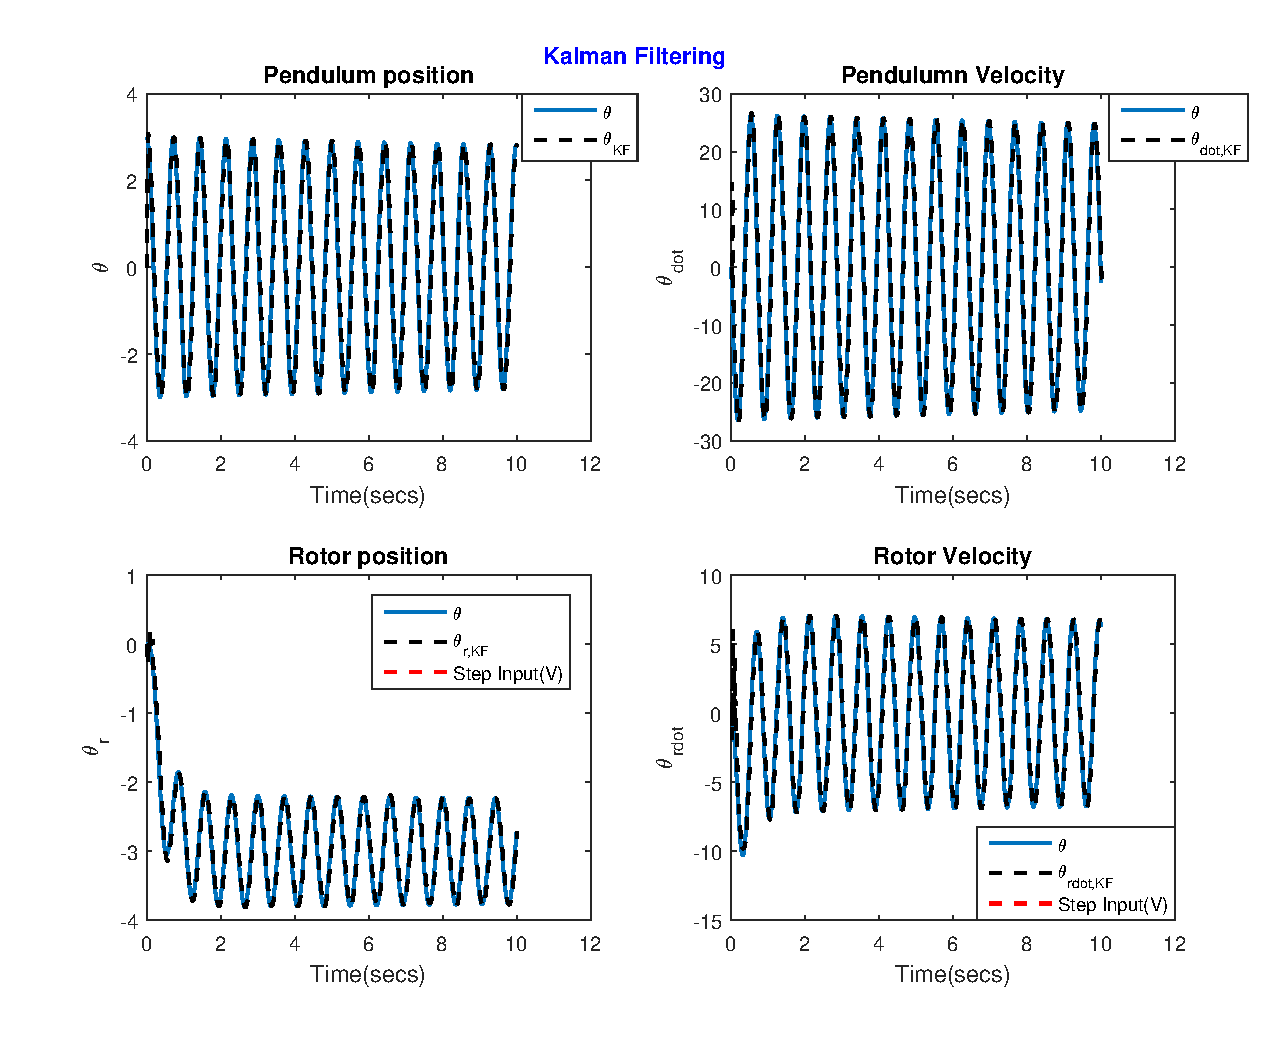
\includegraphics[width=0.7\linewidth]{fig/plot_1_kf3}
	\caption{Initial Condition: $\theta_1 = 3^0$, $\theta_2 = 0$ and no motor pulse applied}
	\label{fig:plot_1_kf3}
\end{figure}
\subsection{Extended Kalman Filtering}

The extended Kalman filter (EKF) is the nonlinear version of the Kalman filter which linearizes about an estimate of the current mean and covariance. With nonlinear systems the Gaussian input doest not necessarily produce a Gaussian output (unlike linear case). Fundamentally assumption in EKF is the estimated state $\hat X$ is close to true state $X$ at all time, and hence the error dynamics can be fairly accurately represented as the linearized plant dynamics about the estimate $\hat X$.\\

The nonlinear system is linearized, as in \ref{eq:19} and \ref{eq:20}
where
\begin{equation}
A = \left[\begin{array}{cccc}
\frac{\partial f_1}{\partial \theta_1}& \frac{\partial f_1}{\partial \theta_2}  &  \frac{\partial f_1}{\partial \theta_3}  & \frac{\partial f_1}{\partial \theta_4}  \\ 
&&&\\
\frac{\partial f_2}{\partial \theta_1}& \frac{\partial f_2}{\partial \theta_2}  &  \frac{\partial f_2}{\partial \theta_3}  & \frac{\partial f_2}{\partial \theta_4}  \\  
&&&\\
\frac{\partial f_3}{\partial \theta_1}& \frac{\partial f_3}{\partial \theta_2}  &  \frac{\partial f_3}{\partial \theta_3}  & \frac{\partial f_3}{\partial \theta_4}  \\ 
&&&\\
\frac{\partial f_4}{\partial \theta_1}& \frac{\partial f_4}{\partial \theta_2}  &  \frac{\partial f_4}{\partial \theta_3}  & \frac{\partial f_4}{\partial \theta_4}  \\  
\end{array} \right]_{x = \hat X(k|k)}  
\label{eq:27}
\end{equation}\\
The above linearized state transition matrix is evaluated at every updated estimate $\hat X(k|k)$. Subsequently the discretized system dynamics $\Phi(k+1,k)$ is evaluated at every time step of estimator using the discretization procedure given in \ref{eq:25} and \ref{eq:26}.\\
\newpage
The Extended-Kalman Filtering is summarized in following table
\begin{center}
	\begin{tabular}{|c|c|}
		\hline & \\
		Model & Dynamics  \\
		& $\dot X = f(x,U,W)$\\
		& Measurement Equation\\
		& $Z(k+1) = HX(k+1)$ \\
		\hline & \\             
		Initialization & $\hat X(k|k) = \hat X(0)$\\ 
		& Error Covariance\\
		& $P(k|k) = E(\tilde X(0) \tilde X(0)^T )$\\
		\hline & \\
		State & $\dot{\hat X} = f(\hat X(k|k),U(k)$  \\ 
		Prediction & RK-4 Integration is used to solve the differential equation \\
		           & for predicted state variable $\hat X(k+1\mid k )$\\
		\hline & \\
		Linearize the system    &  Evaluate A given in \ref{eq:27} at at $X(k|k)$ \\  
		                        &  and discretize the system to evaluate $\Phi(k+1,k)$ \\     
		\hline & \\
		Covarince & $P(k+1|k) = \Phi P(k|k)\Phi ^T + \Gamma Q \Gamma ^T$  \\ 
		propagation & \\
		\hline  &  \\ 
		Kalman  & $K(k+1) = P(k+1|k)H^T(HP(k+1|k)H^T+R)^{-1}$ \\
		Gain Computation            	& \\
		\hline  &  \\
		State Update & $\hat X(k+1|k+1) = \hat X(k+1|k) + K(k+1)(Z(k+1)-H\hat X(k+1|k))$\\
		&  \\ 
		\hline  &  \\ 
		Covariance Update & $P(k+1|k+1) = (I-KH)P(k+1|k)(I-KH)^T + KRK^T$\\
		&  or \\
		& $P(k+1|k+1) = (I-KH)P(k+1|k)$ \\
		\hline
		\end{tabular} 
\end{center}

\subsubsection{Results: Extended Kalman Filtering}
Figure \ref{fig:plot_2_ekf1}, shows the simulation results for very large displacement of the pendulum from the equilibrium position. Since the EKF linearizes the plant the EKF estimate of the state are more accurate compared to linearized kalman filter estimate.\\

Figure \ref{fig:plot_2_ekf_2} and \ref{fig:plot_2_ekf_3} shows the plot with pendulum initial condition in neighborhood of the $0^0$ angle with and without the motor impulse. For this case EKF and KF estimates are comparable because the linearization errors are small and KF also performs good compared to EKF in state estimate. \\

Figure \ref{fig:plot_2_ekf_4} shows the case for initial condition of the pendulum angle to be near upright position thats is $\theta_1 = 150^0$. A well tuned EKF estimates the states very well even when we are operating the system very far away from the equilibrium position. Since the in EKF the system is linearized on the previous updated state estimate the EKF does well in estimating the states where as KF fails. 

\begin{figure}
\centering
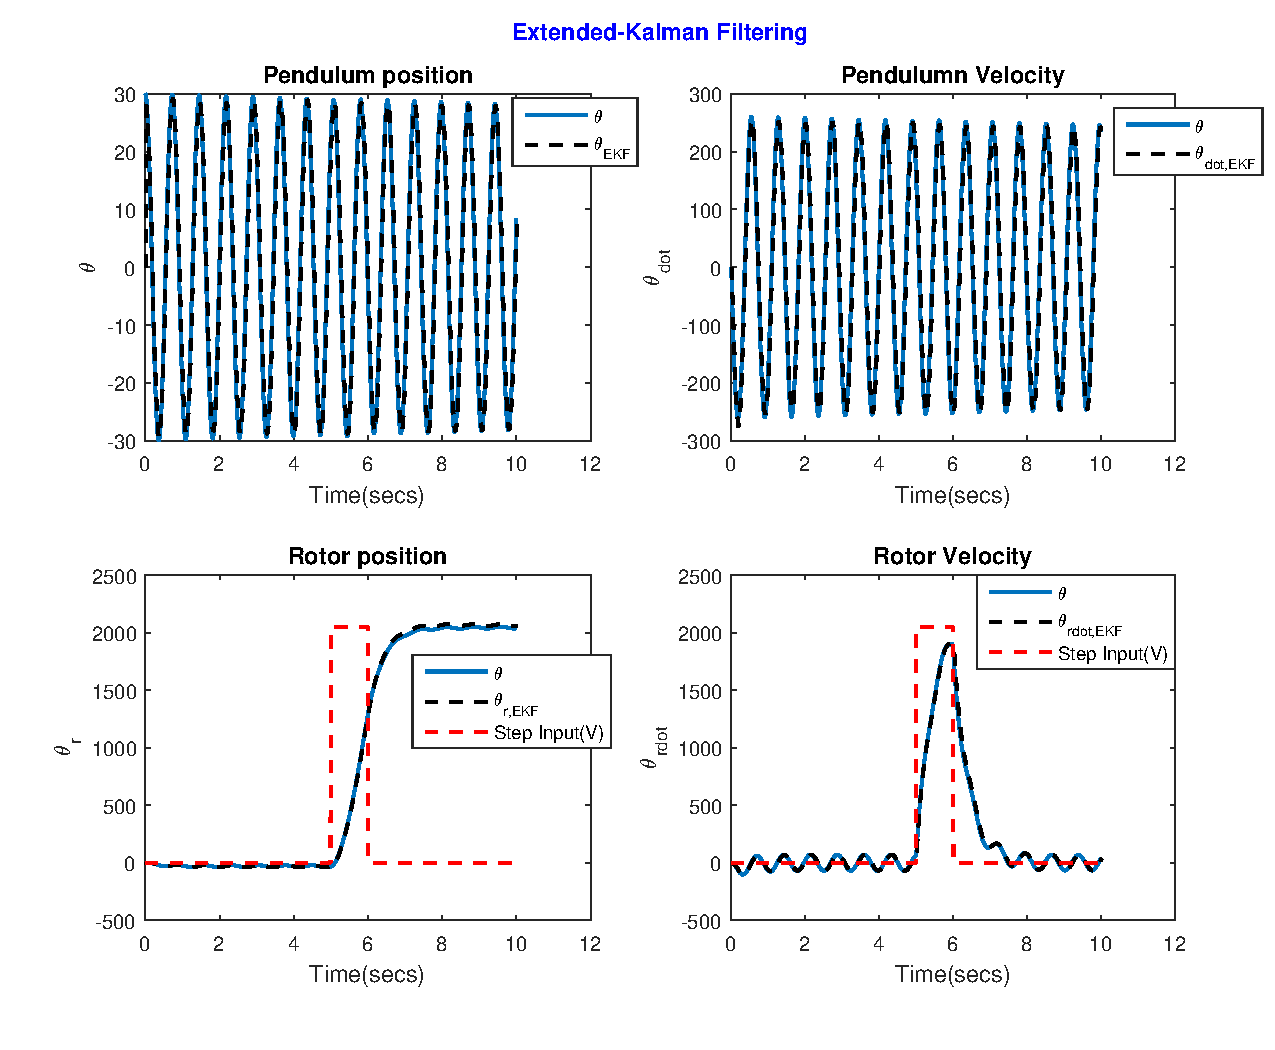
\includegraphics[width=0.7\linewidth]{fig/plot_2_ekf1}
\caption{Initial Condition: $\theta_1 = 30^0$, $\theta_2 = 0$ and motor pulse of 5V is applied at $t = 5secs$}
\label{fig:plot_2_ekf1}
\end{figure}
\begin{figure}
\centering
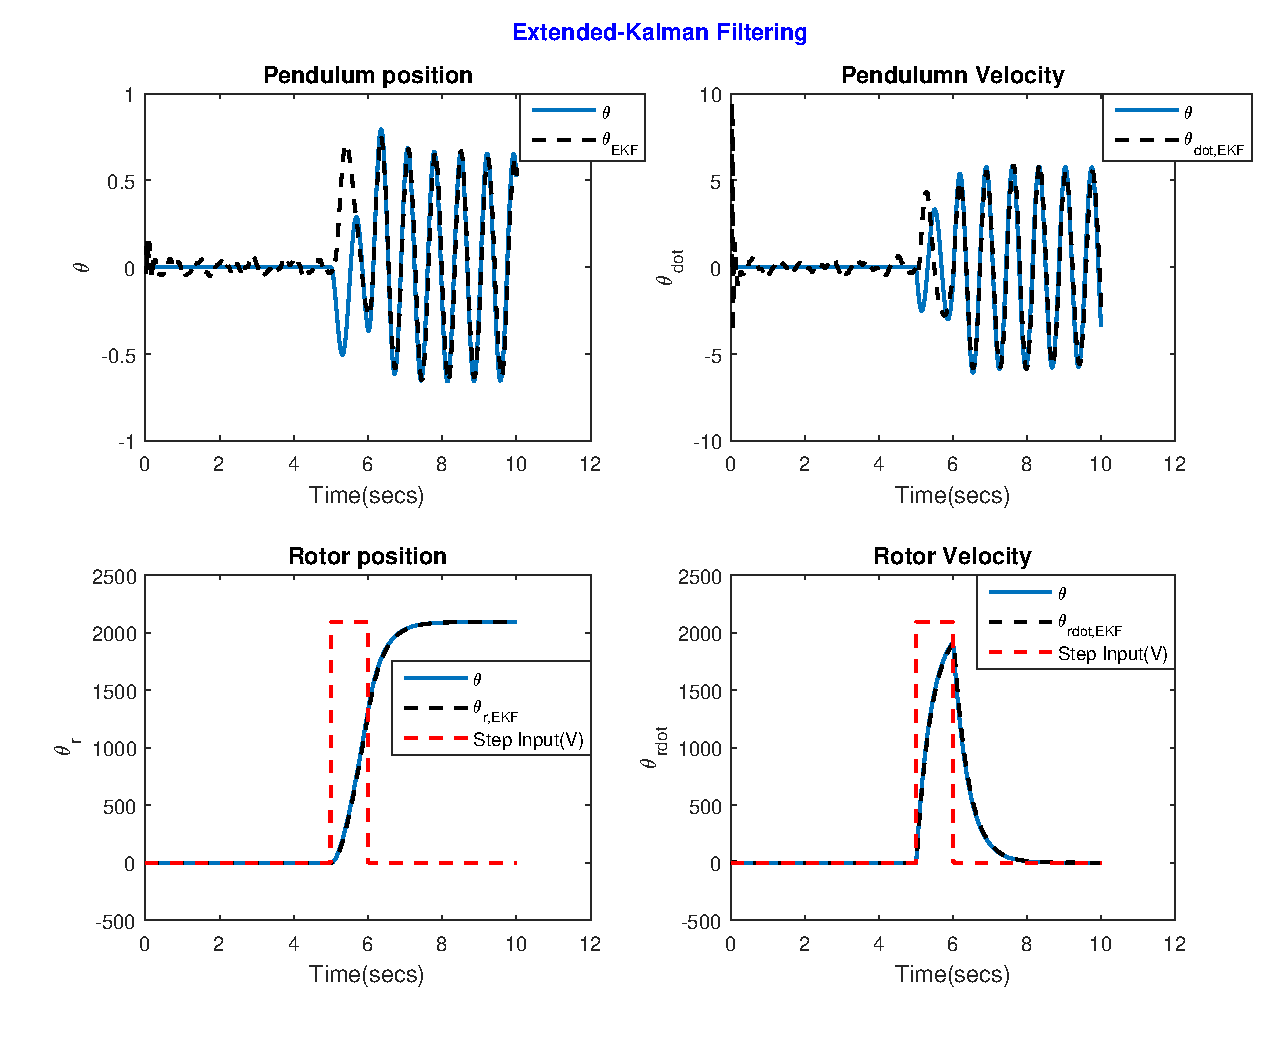
\includegraphics[width=0.7\linewidth]{fig/plot_2_ekf_2}
\caption{Initial Condition: $\theta_1 = 0$, $\theta_2 = 0$ and motor pulse of 5V is applied at $t = 5secs$}
\label{fig:plot_2_ekf_2}
\end{figure}
\begin{figure}
\centering
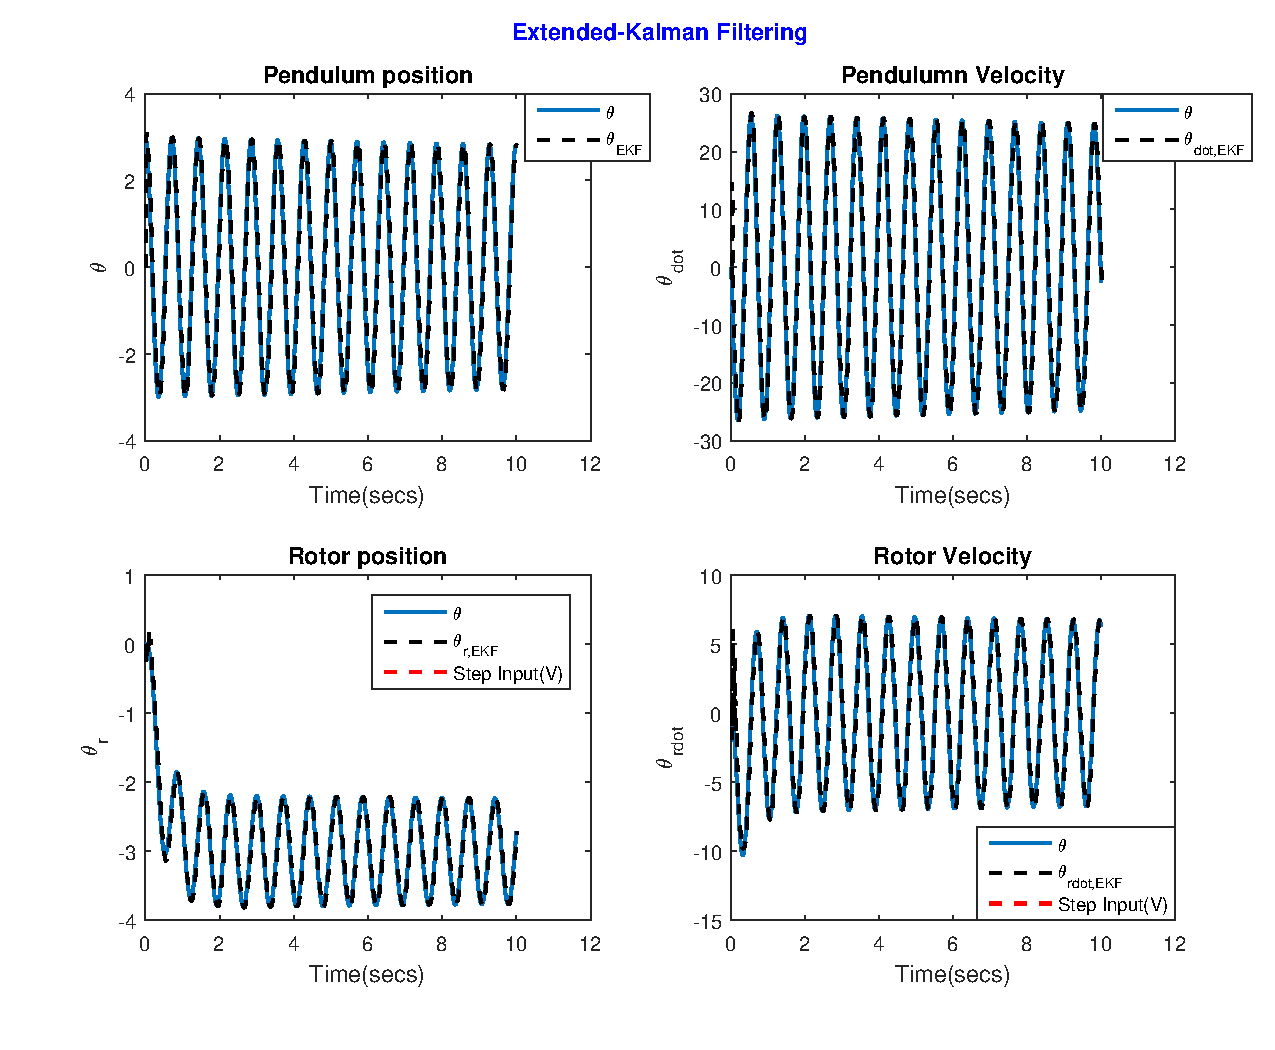
\includegraphics[width=0.7\linewidth]{fig/plot_2_ekf_3}
\caption{Initial Condition: $\theta_1 = 3^0$, $\theta_2 = 0$ and no motor pulse applied}
\label{fig:plot_2_ekf_3}
\end{figure}
\begin{figure}
\centering
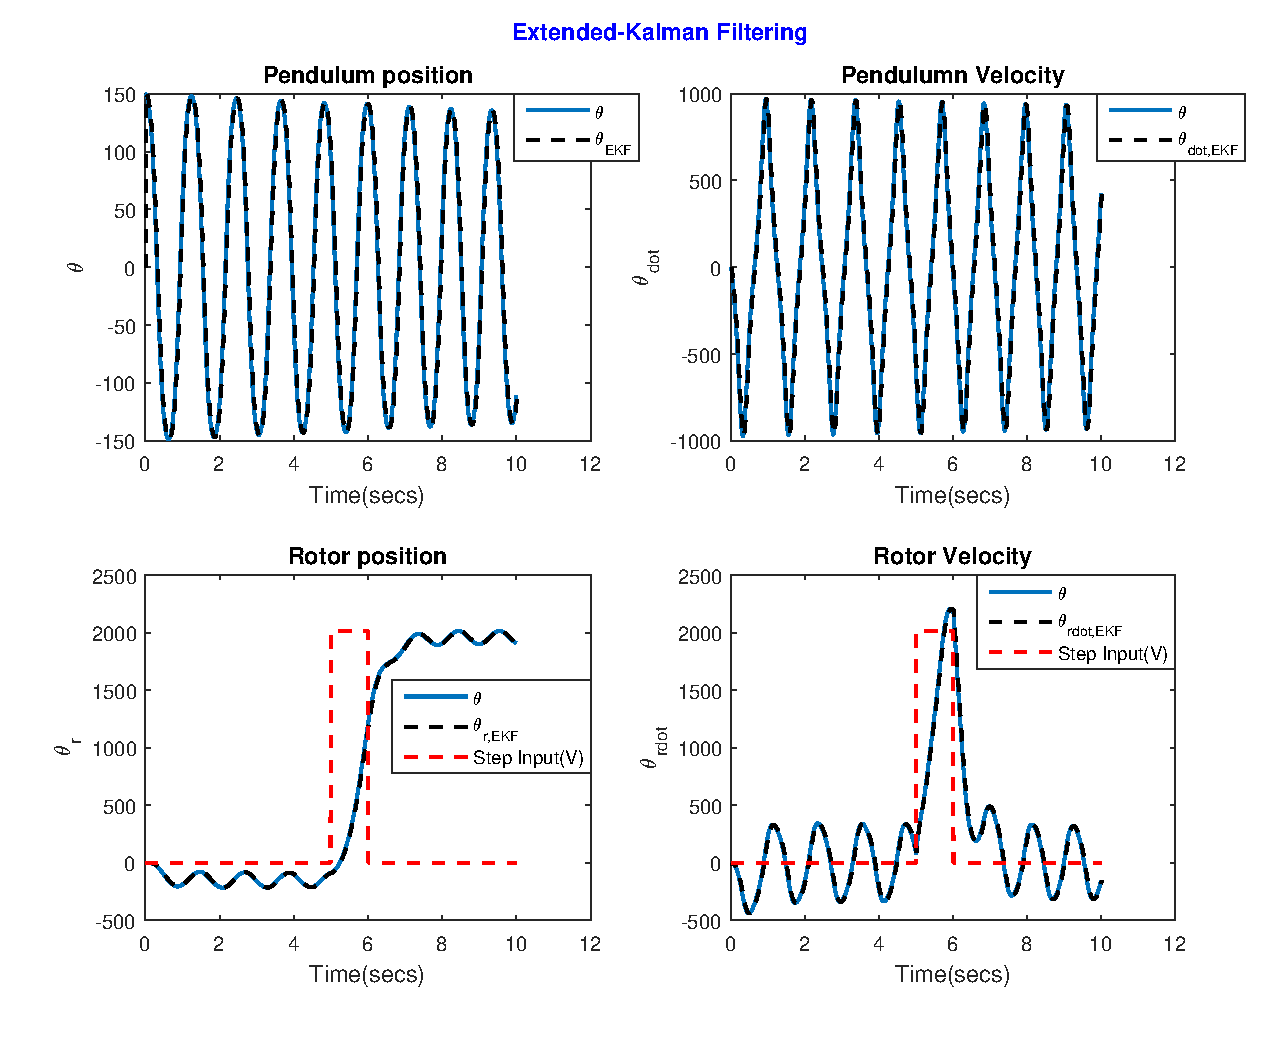
\includegraphics[width=0.7\linewidth]{fig/plot_2_ekf_4}
\caption{Initial Condition: $\theta_1 = 150^0$, $\theta_2 = 0$ and motor pulse of 5V is applied at $t = 5secs$}
\label{fig:plot_2_ekf_4}
\end{figure}

\section{conclusions}
\begin{itemize}
	\item Fundamental assumption in EKF is that true state $X(t)$ is sufficiently close to estimated state $\hat X(t)$, hence the linearized system about $\hat X(t)$ is fairly accurate for state propagation.
	\item Term $P_0$ and $Q$ are tunable parameters and was found that these value needs to be tuned and one single value of $P_0$ and $Q$ does not perform optimally for all the initial conditions.
	\item For initial conditions away from the neighborhood of the stable position, KF performance degrades, where as EKF does well even in the cases where initial conditions for pendulum are near upright positions.
	\item Tuned $Q$ values for EKF are much smaller compared to what need for good performance of the KF.
\end{itemize}
\section{Matlab-codes}
\subsection{Kalman and Extended Kalman Estimate main file and Variable Initialization}
\lstinputlisting{ReactionWheel_Pendulum_Main.m}
\lstinputlisting{Initialization.m}
\subsection{Function File for ODE45 Integration for True Plant Model Propagation}
\lstinputlisting{ReactionWheel_Pendulum.m}
\subsection{Function File for RK-4 Integration for Prediction step of the state}
\lstinputlisting{Reaction_Wheel_Pendulum.m}
\subsection{Function File Results and Plots}
\lstinputlisting{Plots.m}
\end{document} 